%%% Template originaly created by Karol Kozioł (mail@karol-koziol.net) and modified for ShareLaTeX use

\documentclass[a4paper,11pt]{article}

\usepackage[utf8]{inputenc}
\usepackage{graphicx}
\usepackage[usenames,dvipsnames]{xcolor}

\usepackage{tgheros}
%\usepackage[defaultmono]{droidmono}

\usepackage{amsmath,amssymb,amsthm,textcomp}
\usepackage{enumerate}
\usepackage{multicol}
\usepackage{tikz}

\usepackage{geometry}
\geometry{total={210mm,297mm},
left=25mm,right=25mm,%
bindingoffset=0mm, top=20mm,bottom=20mm}


\linespread{1.3}

\newcommand{\linia}{\rule{\linewidth}{0.5pt}}

% custom theorems if needed
% my own titles
\makeatletter
\renewcommand{\maketitle}{
\begin{center}
\vspace{2ex}
{\huge \textsc{\@title}}
\vspace{1ex}
\\
\linia\\
\@author \hfill \@date
\vspace{4ex}
\end{center}
}
\makeatother
%%%

% custom footers and headers
\usepackage{fancyhdr}
\pagestyle{fancy}
\lhead{}
\chead{}
\rhead{}
\lfoot{ADE:Assignment 2}
\cfoot{Page \thepage}
\rfoot{15M54097}
\renewcommand{\headrulewidth}{0pt}
\renewcommand{\footrulewidth}{0pt}
%

% code listing settings
\usepackage{listings}
\lstset{
    language=SQL,
    basicstyle=\ttfamily\small,
    aboveskip={1.0\baselineskip},
    belowskip={1.0\baselineskip},
    columns=fixed,
    extendedchars=true,
    breaklines=true,
    tabsize=4,
    prebreak=\raisebox{0ex}[0ex][0ex]{\ensuremath{\hookleftarrow}},
    frame=lines,
    showtabs=false,
    showspaces=false,
    showstringspaces=false,
    keywordstyle=\color[rgb]{0.627,0.126,0.941},
    commentstyle=\color[rgb]{0.133,0.545,0.133},
    stringstyle=\color[rgb]{01,0,0},
    numbers=left,
    numberstyle=\small,
    stepnumber=1,
    numbersep=10pt,
    captionpos=t,
    escapeinside={\%*}{*)}
}

%%%----------%%%----------%%%----------%%%----------%%%

\begin{document}

\title{Advanced Data Engineering: Assignment 2}

\author{NGUYEN T. Hoang - SID: 15M54097}

\date{Fall 2015, W831 Tue. Period 5-6 \\ \hfill Due date: 2015/10/27}

\maketitle

\section*{Problem}

Consider a data warehouse of a large delivery company (such as FedEx, UPS, DHL). The information generated for each delivery order is stated in the assignment document. For such situation, I consider these following aspect of the desired system: Business model, possible users and actions, and system requirements.

\paragraph{Business model} The operation of the delivery company is assumed and stated simply as follow:
\begin{itemize}
    \setlength{\itemsep}{0cm}
    \setlength{\parskip}{0cm}
    \item Delivery company receives delivery orders and delivery objects from customers.
    \item Delivery company's branches process the delivery orders and execute them.
    \item During delivery, customers can track the delivery status of the package using an web application or mobile application.
    \item Various information about the delivery order will be recorded or queried through out the delivery process.
    \item For each order, there can be only one type of objects, but there can be multiple object in one order. Customers have to place multiple order in case they want to send multiple type of objects.
    \item Delivery company's employees can access the Data Warehouse to do their work.
\end{itemize}

\paragraph{Possible users and actions} The term ``users'' is referred to the company's employees, who has access to the Data Warehouse system only. Their identities and possible actions are:
\begin{itemize}
    \setlength{\itemsep}{0cm}
    \setlength{\parskip}{0cm}
    \item \textbf{Statisticians} are professionals who write complex query \emph{directly} to the Data Warehouse. They perform data analyzing to produce meaningful information about the data to help improving the company's operation. These users are professionals themself, so in the scope of this assignment there will be no consideration for these users. Statisticians have full direct access to the Data Warehouse.
    \item \textbf{Knowledge users} perform queries to quantify each subject area and create reports for other users. They have direct access to some certain parts of the Data Warehouse.
    \item \textbf{Excutives} are managers who perform queries for business administration and decision making. However, they do not need to perform complex queries. Aggregation is the most common query among excutives, and the queries is performed on the reports from knowledge users, not from the Data Warehouse. They use these information to make strategic business decisions. This type of user does not have direct access to the Data Warehouse, but they might have access to the graphic data visulization tool provied by the system.
    \item \textbf{Employees} are deliverypeople or office worker in each branch. Their queries are also performed on the report from knowledge users. They have limited access to the database, and they can only perform basic queries such as queries about a particular package's deliver address. 
    \item \textbf{Customers} can also be a part of the user group. Customers can perform some queries about their orders status (e.g.\ expected delivery date, location, etc.) through a smartphone application or a web application. This type of user has the lowest right of access to the system.
\end{itemize}

\paragraph{System Requirements} Based on the information given in the assignment document and the consideration above, I propose some of the requirements for the Data Warehouse:
\begin{itemize}
    \setlength{\itemsep}{0cm}
    \setlength{\parskip}{0cm}
    \item The system should be responsive for every users' query.
    \item Process power should be able to handle more than 1,200 order per second. (currently, it's 1000 order per second)
    \item The system should be scalable and robust.
    \item Address each business problem correctly and efficiently with each fact table of the star schema.
\end{itemize}



\section*{Question 1}

\textit{Consider other information related to the deliver orders (e.g.\ zip, telephone number \ldots)
    \begin{itemize}
        \setlength{\itemsep}{0cm}
        \setlength{\parskip}{0cm}
        \item They should be different order by order.
        \item Assume also appropriate data size for the information.
    \end{itemize}
} 

\noindent
\textbf{Answer:} Extra information should be added to the delivery orders could be specific time requirements, or regional information for the order.
\begin{multicols}{2}
    \begin{itemize}
        \setlength{\itemsep}{0cm}
        \setlength{\parskip}{0cm}
        \item OrderDay {\color{RoyalBlue}3 BYTE STRING}
        \item OrderDayOfMonth {\color{RoyalBlue}1 BYTE INT}
        \item OrderMonth {\color{RoyalBlue}10 BYTE STRING}
        \item OrderYear {\color{RoyalBlue}2 BYTE INT}
        \item RequiredDay {\color{RoyalBlue}3 BYTE STRING}
        \item RequiredDayOfMonth {\color{RoyalBlue}1 BYTE INT}
        \item RequiredMonth {\color{RoyalBlue}10 BYTE STRING}
        \item RequiredYear {\color{RoyalBlue}2 BYTE INT}
        \item ShippedDay {\color{RoyalBlue}3 BYTE STRING}
        \item ShippedDayOfMonth {\color{RoyalBlue}1 BYTE INT}
        \item ShippedMonth {\color{RoyalBlue}10 BYTE STRING}
        \item ShippedYear {\color{RoyalBlue}2 BYTE INT}
        \item PhoneNumber {\color{RoyalBlue}15 BYTE STRING}
        \item Fax {\color{RoyalBlue}15 BYTE STRING}
        \item CustomerPhone {\color{RoyalBlue}15 BYTE STRING}
        \item CustomerTitle {\color{RoyalBlue}5 BYTE STRING}
        \item CustomerAddr {\color{RoyalBlue}100 BYTE STRING}
        \item CompanyName {\color{RoyalBlue}50 BYTE STRING}
        \item DstCity {\color{RoyalBlue}20 BYTE STRING}
        \item DstRegion {\color{RoyalBlue}15 BYTE STRING}
        \item DstPostalCode {\color{RoyalBlue}15 BYTE STRING}
        \item DstCountry {\color{RoyalBlue}20 BYTE STRING}
        \item CurrLoc {\color{RoyalBlue}20 BYTE STRING}
        \item OrderStatus {\color{RoyalBlue}1 BYTE INT}
    \end{itemize}
\end{multicols}

\section*{Question 2}

\textit{Depict your star schema to store the deliver order information including your own assumptions for \textbf{Question 1}.} 

\noindent
\textbf{Answer:} I propose a star schema as in figgure 1 below. In my design I use a factless fact table contains only keys to the dimention tables. The reason for me to choose this design is that a factless fact table can give better description about the delivery busines and the flexibility of the design. For example, using a factless fact table, the system can answer queries about both number of packages delivered in a period of time and the time it takes for a package to be delivered
or even aggregation queries about customers. Also, I made design decision for data size of each attributes in the table. I considered the number of operations and performance (such as sorting) that the system should handle frequently.

\vspace{3em}

\begin{figure}[htbp]
    \centering
    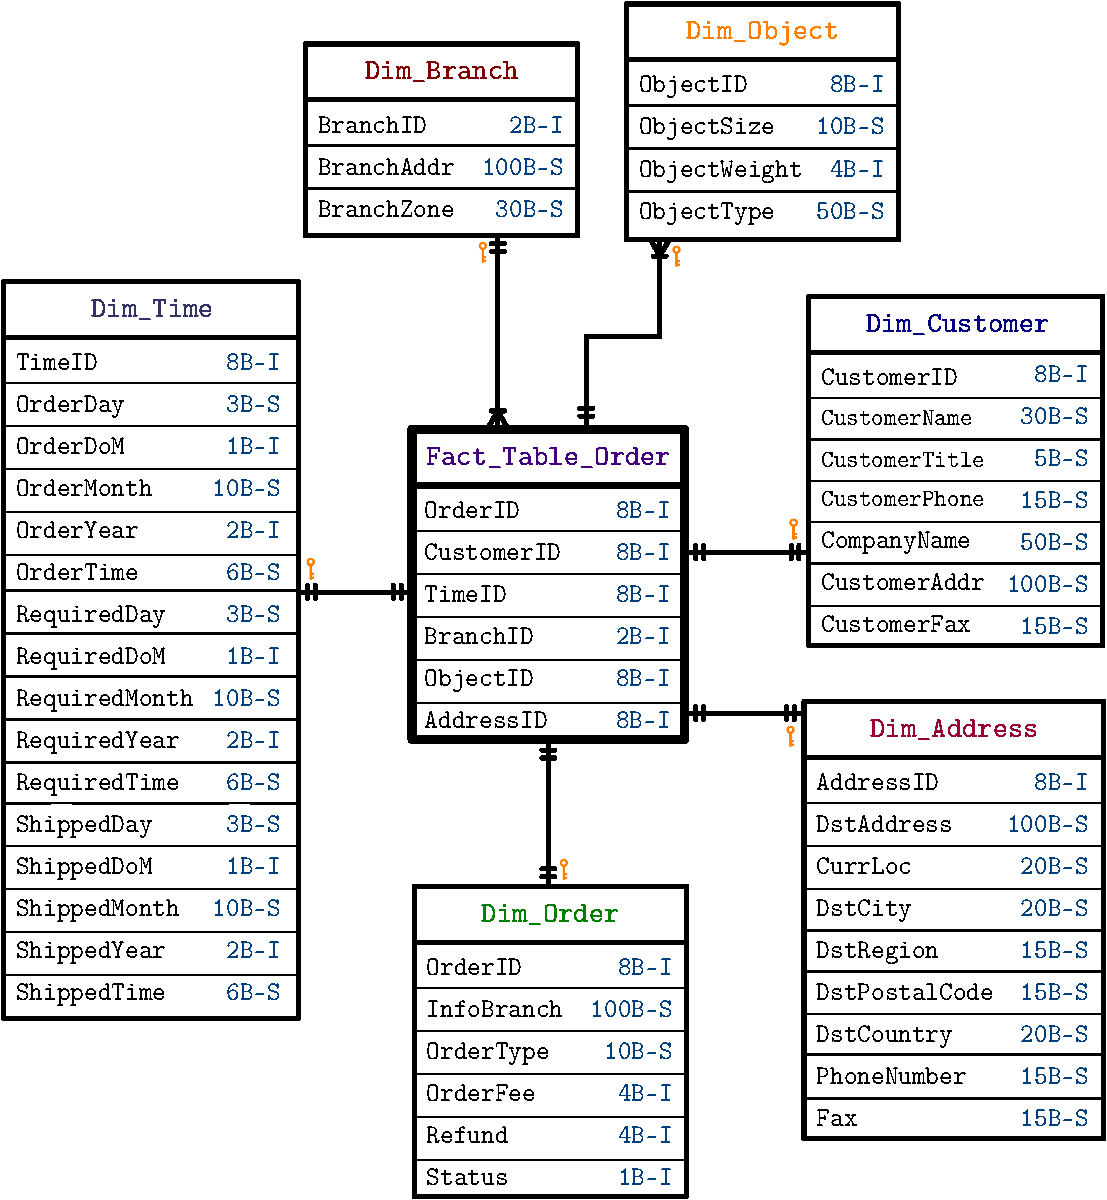
\includegraphics[scale=0.75]{OrderStarSchema.pdf}
    \caption{Star Schema for Deliver Orders}
\end{figure}

\pagebreak

\section*{Question 3}

\textit{Calculate the amount of data stored in the data warehouse using the star schema of \textbf{Question 2} for a day.} 

\noindent
\textbf{Answer:} Base on the proposed star schema in Figure 1, the data size calculation for one day is done as follow: 
\begin{itemize}
    \setlength{\itemsep}{0cm}
        \setlength{\parskip}{0cm}
    \item The size of Dim\_Branch is ignored since Dim\_Branch contains total of 10,000 records, independent with the number of orders.
    \item Data size for each order is the sum of all size of attributes in the fact table and dimension table.
    \item Total data size for one day is the size of each order times with number of order per day.
\end{itemize}

\noindent
Number of order per day:
\vspace{-0.75em}
$$N_{orders}=R_{orders\_per\_sec}\times Seconds\ In\ A\ Day$$
$$N_{orders}=1000 \times 86400=86.4\times 10^{6}\ orders$$
Data size for each order:
$$Size_{deliver\_order}=Size_{Fact}+Size_{Time}+Size_{Order}+Size_{Address}+Size_{Customer}+Size_{Object}$$
$$Size_{deliver\_order}=42+74+127+228+223+72=766\ Bytes$$
Data stored in the data warehouse using the proposed star schema for a day:
$$DataSize_{1\_day}=N_{orders}\times Size_{deliver\ order}$$
$$DataSize_{1\_day}=86.4\times 10^{6}\times 766=66,182,400,000\ Bytes$$
$$DataSize_{1\_day}\approx\ 66\ GB$$

\section*{Question 4}

\textit{Calculate the increase of data amount for a year.} 

\noindent
\textbf{Answer:} Not taking leap year into account, a year has 365 days.
The amount of data will be increased over a year with the proposed star schema:
\vspace{-0.75em}
$$DataSize_{1\_year}=DataSize_{1\_day}\times 365=66,182,400,000\times 365$$
$$DataSize_{1\_year}=24,156,576,000,000\ Bytes\approx 24\ TB$$

\section*{Question 5}

\textit{Consider the situation without using star schema; you use a big table containing all attributes, and compare with the star scheme you defined for \textbf{Question 2}.} 

\noindent
\textbf{Answer:} Assume that the big table containing all attributes omits all redundancy ID attributes to make a big table. The size of each order with such assumption is calculated by subtracting twice the size of fact table (each ID appear twice in the star schema), and adding back the size of the OrderID (8) along with the size of BranchID (2).
\vspace{-0.75em}
$$SizeTable_{deliver\_order}=Size_{deliver_order}-2\times Size_{Fact}+8+2=692\ Bytes$$
$$SizeTable_{1\_year}=SizeTable_{1\_day}\times 365=59,788,800\times 365$$
$$SizeTable_{1\_year}=21,822,912,000\ Bytes\approx 22\ TB$$
\noindent
By considering the data size increase over a year and architecture of both ``big table'' and proposed star schema, I can conclude the advantages and disadvantages of both scheme as follow:
\begin{enumerate}
    \setlength{\itemsep}{0cm}
    \setlength{\parskip}{0cm}
\item Normalized big table
    \begin{itemize}
     \setlength{\itemsep}{0cm}
    \setlength{\parskip}{0cm}
\item \textbf{Advantages} of this scheme is that it saves storage space (21 TB over a year versus 24 TB over a year). This scheme is also simpler to understand.
\item \textbf{Disadvantages} of this scheme is that it may handle join operations and changes poorly due to the nature of the big table. 
     \end{itemize}  
 \item Proposed Star Schema
    \begin{itemize}
     \setlength{\itemsep}{0cm}
    \setlength{\parskip}{0cm}
\item \textbf{Advantages} of this scheme is that it has simple design. Moreover, star scheme can handle faster queries, join operation, and better compatible with OLAP model than the aforementioned big table schema. 
\item \textbf{Disadvantages} of this scheme is that it has higher storage because of data denormalization
     \end{itemize}  
    
\end{enumerate}
\section*{Question 6}

\textit{Consider an SQL sentence to derive the total weight of the objects of which type is fresh foods, shipped by branches in Kansai zone for this year from the star schema of \textbf{Question 2}.} 

\noindent
\textbf{Answer:} 
\vspace{-1.5em}
\begin{lstlisting}[label={list:first},caption=SQL sentence for total weight of `Fresh foods' delivered in `Kansai' this year (2015)]
SELECT SUM(ObjectWeight)
FROM Dim_Object
WHERE 
    ObjectID IN (
        SELECT ObjectID
        FROM Fact_Table_Order
        WHERE BranchID IN (
            SELECT BranchID
            FROM Dim_Branch
            WHERE BranchZone = 'Kansai')
        AND TimeID IN (
            SELECT TimeID
            FROM Dim_Time
            WHERE ShippedYear = 2015))
    AND ObjectType = 'Fresh foods';
\end{lstlisting}

\end{document}
